%% Noch anders strukturieren!!

\section{GPS}

Die GPS-Daten wurden von Alexandra ausgelesen und uns als Tabelle zur Verfügung gestellt. Diese ist in der Gesamtübersicht zu finden. ??? Damit konnte dann eine Übersichtskarte des Messgebiets erstellt werden, die auch in die Gesamtübersicht aufgenommen wurde.

\section{Tachymetrie}

Mit der Tachymetrie wurde die Höhe der einzelnen Messpunkte relativ zu einer Totalstation vermessen. Diese werden für die Freiluft- und Bouguerreduktion benötigt.

%Tachymeter-Tabelle auch hier rein?

\section{Reduktionen}

Nach den bereits im Feld durchgeführten Reduktionen wurde noch am Versuchstag die Driftkorrektur mit dem zur Verfügung gestellten MATLAB-Programm GDRIFT durchgeführt. Da beim zweiten Durchlauf der mit Gravimeter 156G am Punkt G2 aufgenommene Wert sehr große Abweichungen zeigte, wurde dieser bei der Interpolation nicht berücksichtigt. Das gleiche war bei G15 und Gerät 686G der Fall. Beide Werte wurden dennoch korrigiert und dann weiter verwendet. Die Driftkurven sind in den Abbildungen \ref{fig:drift1} und \ref{fig:drift2} abgebildet. Nach Abzug der Drift von den einzelnen Messwerten, wurde der Mittelwert der beiden Messreihen für jedes Gravimeter gebildet. Nun wurden die Messreihen der beiden Gravimeter zusammen geführt, um das vollständige driftkorrigierte Profil zu erhalten. Dabei wurde das Offset der beiden Gravimeter zueinander am Basispunkt G0 berücksichtigt. Da nur der relative Unterschied dieser Werte relevant ist, wird der kleinste Messwert von allen abgezogen.
%Diese Werte werden im folgenden mit $\Delta \q{g}{driftkorr}$ bezeichnet.

\begin{figure}[!ht]
 \centering
 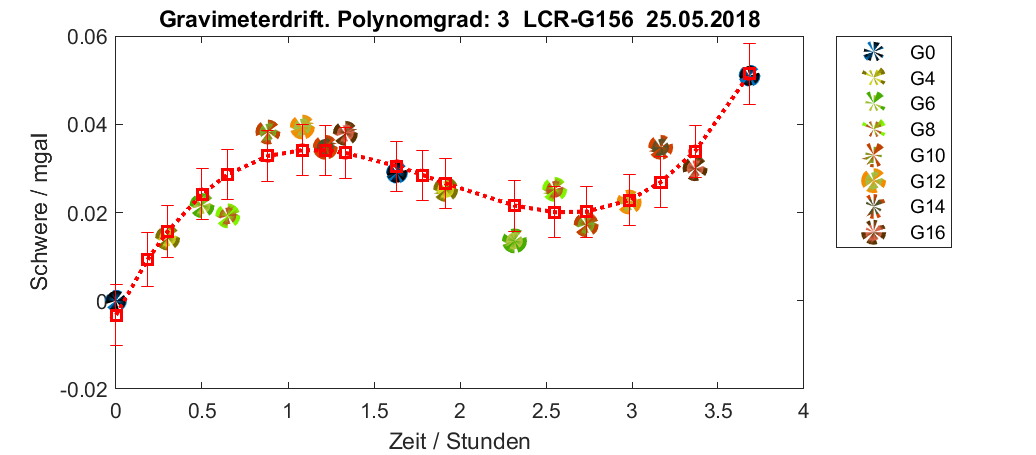
\includegraphics[width=0.8\textwidth]{fig/G156drift_endgultig}
 \caption[Gravimeterdrift des Geräts 156G]{Gravimeterdrift des Geräts 156G. Die Messwerte an Punkt G2 wurden für die Bestimmung der Driftkurve nicht verwendet, weil sie zu starke Abweichungen zeigten.}
 \label{fig:drift1}
\end{figure}

\begin{figure}[!ht]
 \centering
 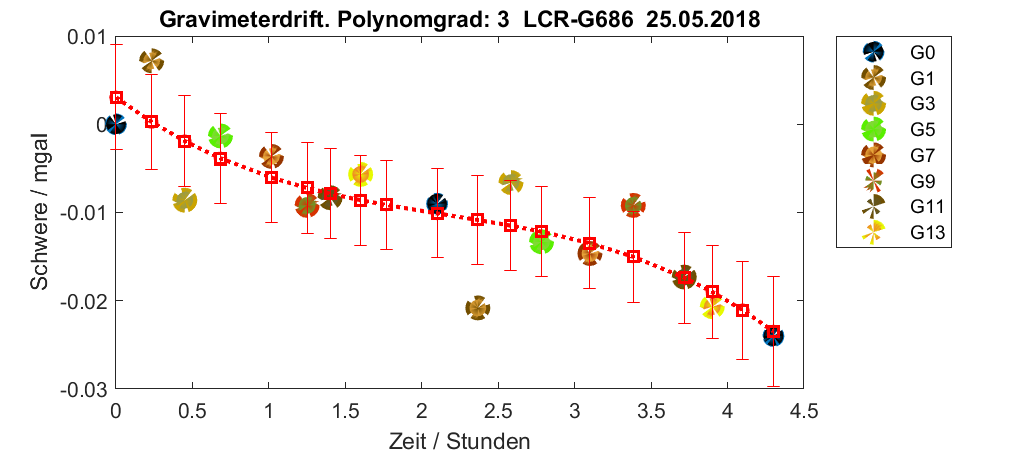
\includegraphics[width=0.8\textwidth]{fig/G686drift_endgultig}
 \caption[Gravimeterdrift des Geräts 686G]{Gravimeterdrift des Geräts 686G. Die Messwerte an Punkt G15 wurden für die Bestimmung der Driftkurve nicht verwendet, weil sie zu starke Abweichungen zeigten.}
 \label{fig:drift2}
\end{figure}

An diesen Werten werden die weiteren Korrekturen mit einem python-Skript durchgeführt. Es werden jeweils die Formeln aus Kapitel \ref{sec:Reduktionen} verwendet. In Tabelle \ref{tab:reduktionen} sind diese Reduktionen und die daraus resultierende Bougueranomalie aufgeführt. Für die Bouguer-Plattenreduktion wurde eine Dichte von $\rho=\eb{2500}{kg}{m^3}$ verwendet, weil Dichten von $\eb{2400}{kg}{m^3}$ bis $\eb{2500}{kg}{m^3}$ oft bei gravimetrischen Messungen mit dem Nettleton-Verfahren im Hegau bestimmt werden. Allgemein ist dies aber ein sehr großer Wert für eine Bodendichte. Die Dichte wurde so hoch gewählt, weil dann die Verkippung der Bougueranomlie geringer wurde und so der Einfallswinkel nicht so groß gewählt werden musste.

%Höhe, Rechtswert, ... in eine Tabelle

%Zwischenergebnisse (driftreduzierte, relative Werte...)

% ??? Tabelle mit allen Reduktionen, driftkorrigierte Wetrte...
% Boueguer-Reduktion neu!
\begin{landscape}
\begin{table}[!ht]
\centering
\caption{Werte der durchgeführten Reduktionen und Wert der resultierenden Bougueranomalie}
\label{tab:reduktionen}
\begin{tabular}{llllllll}
\toprule
Messpunkt & Profilkoordinate in m & $\q{\delta}{g\,Bouguer}$ in mGal & $\q{\delta}{g\,Niv}$ in mGal & $\q{\delta}{g\,Breite}$ in $\upmu$Gal & $\q{\delta}{g\,geol}$ in $\upmu$Gal & $\q{\delta}{g\,Gel}$ in mGal & $\q{g}{Bouguer}$ in mGal \\
\midrule
G0 & 0.000 & 0.000 & 0.000 & 0.00 & 0.000 & -0.701 & 1.444 \\
G1 & 7.952 & 0.042 & -0.136 & 3.13 & -0.200 & -0.707 & 1.415 \\
G2 & 14.929 & 0.097 & -0.310 & 5.97 & -0.236 & -0.71 & 1.424 \\
G3 & 20.897 & 0.141 & -0.453 & 8.32 & -0.376 & -0.711 & 1.456 \\
G4 & 25.860 & 0.187 & -0.599 & 10.36 & -0.364 & -0.715 & 1.472 \\
G5 & 29.780 & 0.216 & -0.693 & 11.92 & -0.444 & -0.715 & 1.475 \\
G6 & 32.799 & 0.246 & -0.788 & 13.09 & -0.540 & -0.717 & 1.516 \\
G7 & 34.825 & 0.270 & -0.865 & 13.91 & -0.568 & -0.717 & 1.548 \\
G8 & 36.842 & 0.293 & -0.938 & 14.79 & -0.482 & -0.717 & 1.567 \\
G9 & 39.792 & 0.325 & -1.042 & 15.99 & -0.489 & -0.719 & 1.543 \\
G10 & 43.761 & 0.360 & -1.154 & 17.65 & -0.444 & -0.721 & 1.546 \\
G11 & 48.741 & 0.404 & -1.294 & 19.64 & -0.516 & -0.722 & 1.512 \\
G12 & 54.697 & 0.446 & -1.429 & 22.10 & -0.487 & -0.725 & 1.511 \\
G13 & 61.658 & 0.496 & -1.587 & 24.88 & -0.611 & -0.73 & 1.502 \\
G14 & 69.585 & 0.560 & -1.792 & 28.11 & -0.640 & -0.733 & 1.506 \\
G15 & 78.549 & 0.643 & -2.059 & 31.73 & -0.721 & -0.738 & 1.480 \\
G16 & 84.602 & 0.743 & -2.379 & 34.19 & -0.751 & -0.744 & 1.602 \\ \bottomrule
\end{tabular}
\end{table}
\end{landscape}

\section{Modellierung mit MATLAB}

Nun kann die Modellierung mit MATLAB durchgeführt werden. In Abbildung \ref{fig:Bougueranomalie} ist die resultierende Bougueranomalie abgebildet. Es fällt auf, dass der letzte Wert sehr groß ist und nicht zu den anderen abfallenden Werten am Rand der Anomalie passt. Es wurde dann nochmal für diesen Punkt die gesamte Rechnung überprüft, um einen Auswertungsfehler ausschließen zu können. Da kein Fehler gefunden werden konnte und ein Ausreißer bei einem Profil mit so wenig Messdaten einen großen Einfluss auf das Ergebnis hat, wird der letzte Messwert bei den Modellierungen in MATLAB nicht mit verwendet. 

\begin{figure}[!ht]
 \centering
 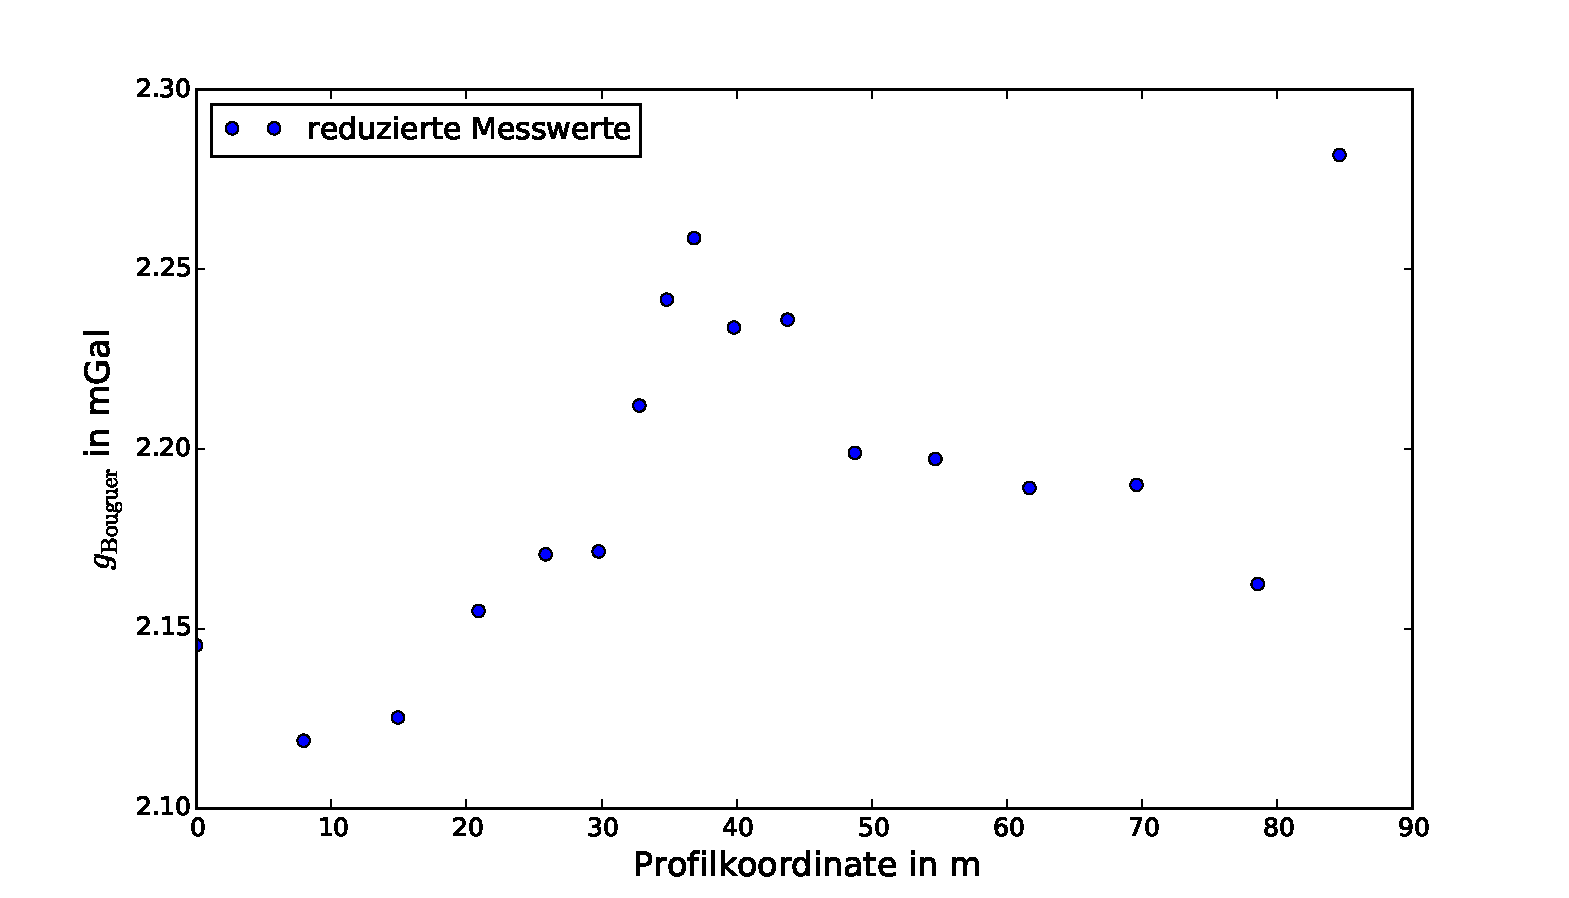
\includegraphics[width=0.7\textwidth]{fig/Plot_Bouguer_mit_letztem_Punkt}
 \caption{Bougueranomalie in Abhängigkeit der Profilkoordinate}
 \label{fig:Bougueranomalie}
\end{figure}

Beim Modellierungs-Programm kann zwischen Spaltenintrusion und Basaltfluss gewählt werden und dann noch viele Parameter eingegeben werden. Deswegen können prinzipiell bei beiden Modellen unendlich viele Untergrundmodelle gefunden werden, die die Messwerte erklären würden. Im folgenden sind einige resultierende Modelle beschrieben.
%Mit Kati und Niels zusammen

Bei beiden Optionen müssen vor der Modellierung einige Parameter abgeschätzt und eingegeben werden. Der Winkel zwischen Messprofil und Streichrichtung des Störkörpers konnte mit der Magnetik-Kartierung sehr genau zu 90$^\circ$ bestimmt werden, weswegen dies für alle Profile so gewählt wurde. Außerdem muss immer der mittlere Fehler der Beobachtungen angegeben werden. Um nicht einen zu kleinen Fehler anzugeben, wurde hier für beide Messgeräte der größte Fehler benutzt, welcher in Gleichung \eqref{eq:Fehler} in Kapitel \ref{sec:Fehler} berechnet wird. Die Tiefenerstreckung des Störkörpers wurde auf 1000\,m gesetzt, weil der Riedheimer Basaltgang in einer geologischen Karte bei einem Schnitt so tief wie dieser eingezeichnet ist. Es muss auch immer die Profillage des Schweremaximums, also der Mittelpunkt der Anomalie eingegeben werden. Dieser ist aus den Werten der Magnetik-Profile zu schließen bei 37\,m, also Profilpunkt G7. Es wurde zweimal entlang genau des gleichen Profils gemessen und drei mal in einem Abstand von nur 2\,m in beide Richtungen versetzt. Wird das Schweremaximum jedoch immer auf 37\,m gesetzt, erklären die Modelle die Beobachtung häufig nicht gut. Dieser Wert wird also bis zu 3\,m in den folgenden Modellen verschoben.

\subsection{Spaltenintrusion}

Da die Bougueranomalie etwas gekippt aussieht, muss für die Modellierung entweder ein linearer Trend angenommen werden oder davon ausgegangen werden, dass sie schräg einfällt. Für beide Varianten wurden Modelle erstellt.

\subsubsection{Modell 1}

Für dieses Modell wurde der Einfallwinkel (Einfallen) als 120$^\circ$ von West nach Ost gemessen angenommen, da Modelle mit einem geringeren Einfallen die Werte noch nicht gut genug erklärten. Die Option der Schätzung eines linearen Trends wurde für dieses Modell nicht verwendet, weil dieser und der Einfallwinkel nicht unabhängig voneinander bestimmbar sind. Die Ergebnisse sind in Abbildung \ref{fig:modell1} und \ref{fig:modell1_res} dargestellt.

\begin{figure}[!ht]
 \centering
 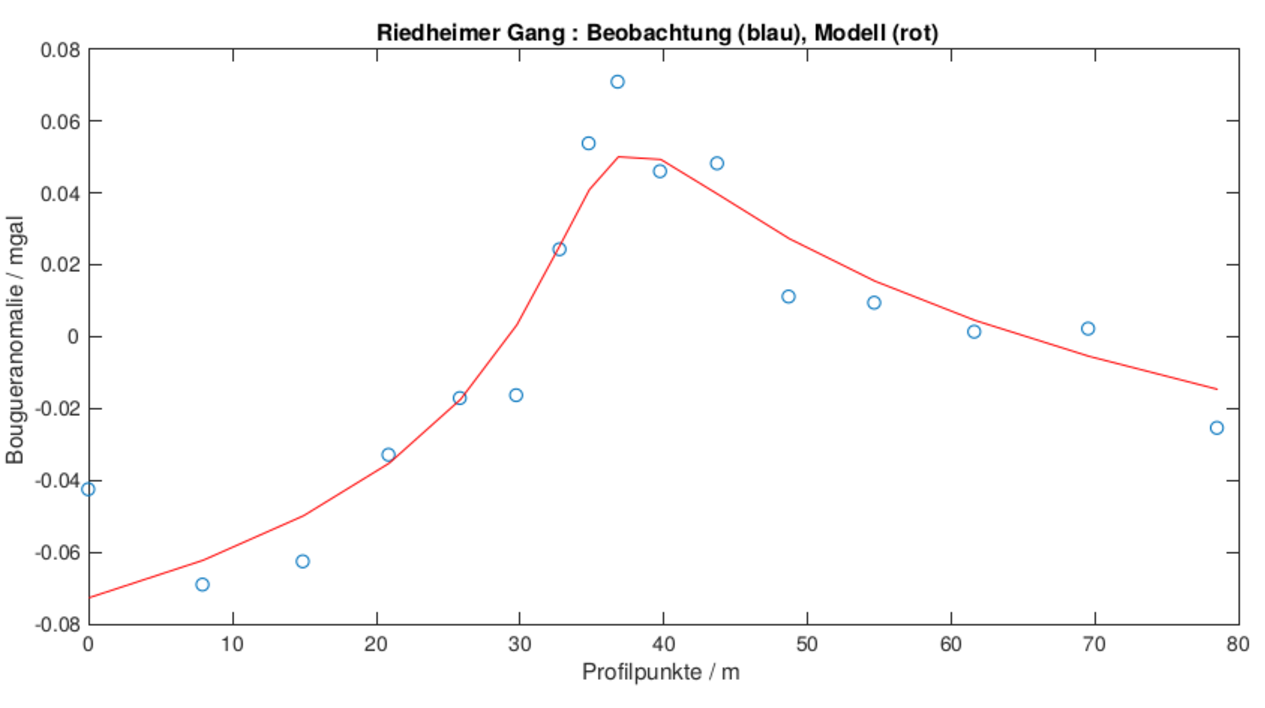
\includegraphics[width=0.8\textwidth]{fig/modell1}
 \caption{Bougueranomalie des ersten Modells}
 \label{fig:modell1}
\end{figure}

\begin{figure}[!ht]
 \centering
 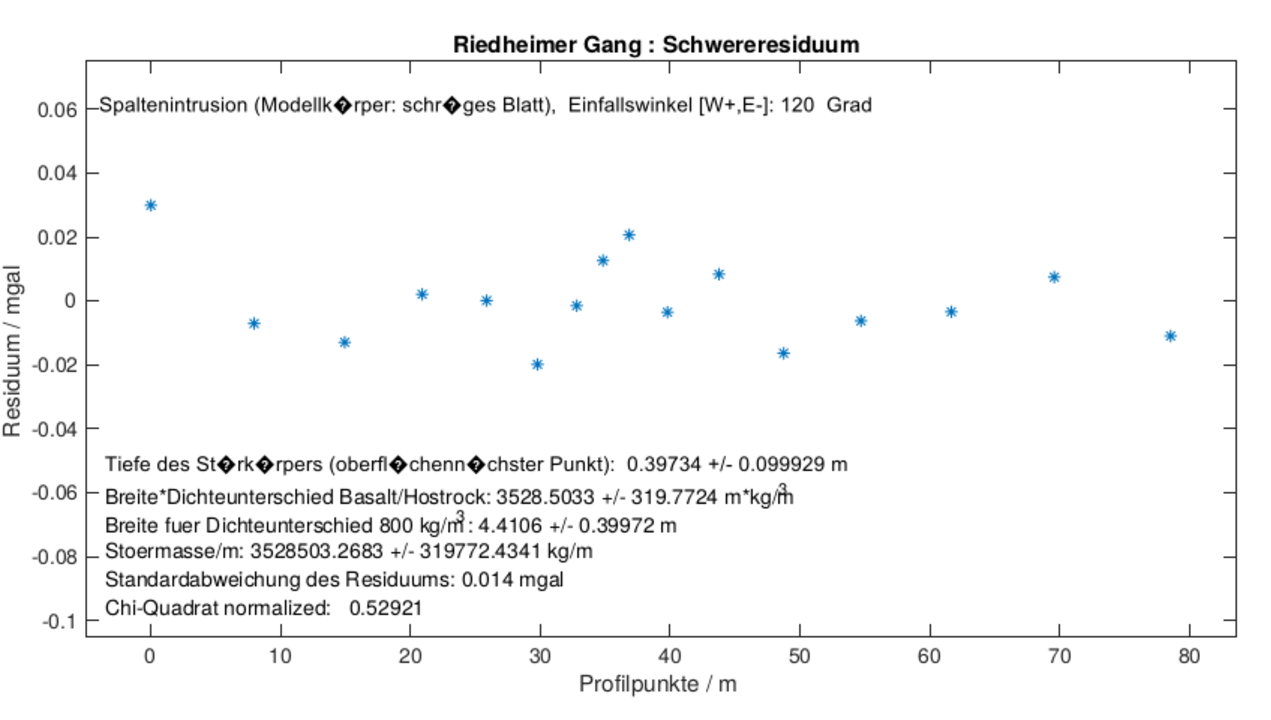
\includegraphics[width=0.8\textwidth]{fig/modell1_res}
 \caption{Schwereresiduudm des ersten Modells}
 \label{fig:modell1_res}
\end{figure}

Der Einfallwinkel scheint mit 120$^\circ$ doch sehr groß zu sein. In der Magnetik wurde zwar auch bestimmt, dass es sich um einen schrägen Gang handeln muss, jedoch ergaben sich Winkel um die 10$^\circ$ bis 20$^\circ$ gemessen von der Senkrechten aus. Die hier angenommenen 30$^\circ$ weichen stark davon ab. Der Eingabewert des oberflächennächsten Punkts der Anomalie 1,5\,m wurde verändert und eine neue Tiefe von $\e{(0,397\pm0,010)}{m}$ berechnet.

\subsubsection{Modell 2}

Nun wurde der Einfallswinkel auf 90$^\circ$ gesetzt und dafür die Option des linearen Trends gewählt, weil nur so die verkippt aussehenden Messwerte modelliert werden können (Ergebnisse siehe Abbildung \ref{fig:modell2} und \ref{fig:modell2_res}). Ein großer Unterschied ist, dass die Tiefe, die wie bei Modell 1 auf 1,5\,m gesetzt wurde, im Ergebnis unverändert bleibt. Es scheint also tatsächlich die eingegebene Tiefe für die Berechnungen genommen zu werden. Sie wurde auf 1,5\,m gesetzt, weil dies der Oberkante der Anomalie im spezifischen Widerstand in der Tomographie auf dem gleichen Profil ergab.

\begin{figure}[!ht]
 \centering
 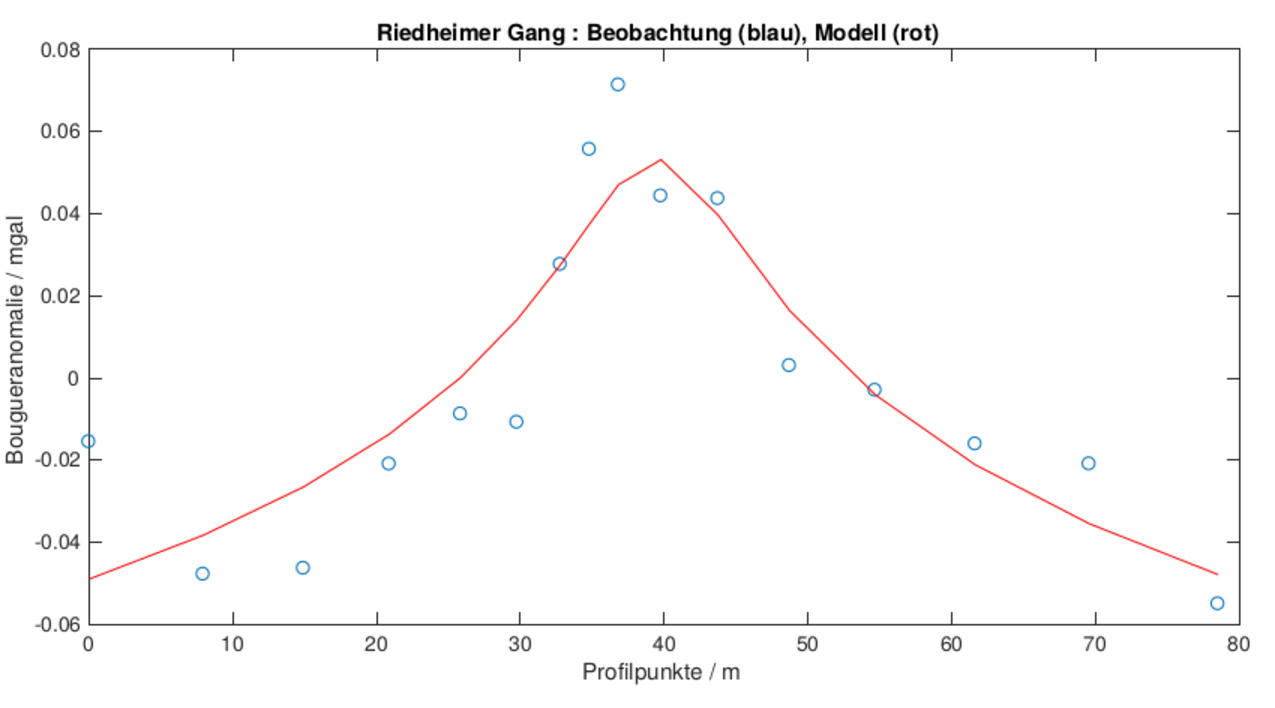
\includegraphics[width=0.8\textwidth]{fig/modell2}
 \caption{Bougueranomalie des zweiten Modells}
 \label{fig:modell2}
\end{figure}

\begin{figure}[!ht]
 \centering
 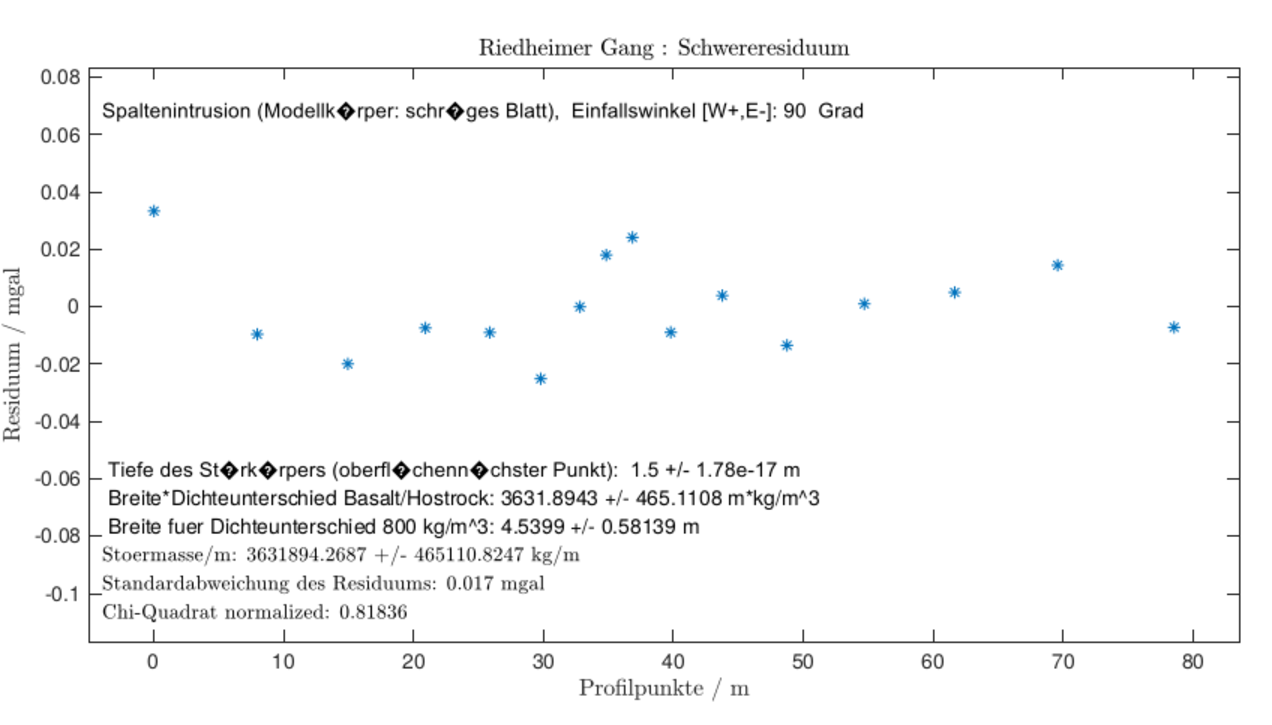
\includegraphics[width=0.8\textwidth]{fig/modell2_res}
 \caption{Schwereresiduudm des zweiten Modells}
 \label{fig:modell2_res}
\end{figure}

\subsection{Basaltfluss}



% \begin{figure}[!ht]
%  \centering
%  \includegraphics[width=\textwidth]{fig/}
%  \caption{}
%  \label{fig:}
% \end{figure}